\chapter{Extra-Credit Question-3}
\label{intro}

\textbf{Rank the 1,682 movies according to the 1997/1998 MovieLense data.  Now rank the same 1,682 movies according to todays (March 2016) IMDB data (break ties based on number of users, for example: 7.2 with 10,000 raters $>$ 7.2 with 9,000 raters).\\
Draw a graph, where each dot is a film (i.e., 1,682 dots).  The x-axis is the MovieLense ranking and the y-axis is today's IMDB
ranking. \\
What is Pearon's r for the two lists (along w/ the p-value)?  Assuming the two user bases are interchangable (which might not be a good
assumption), what does this say about the attitudes about the films after nearly 20 years?}\\


Following are the steps I have taken to solve the problem:

\begin{itemize}
\item I ranked all the movies based on MovieLense. The python code for this is illustrated in \ref{lst:q5code1}
\item Futhermore I ranked all the movies based on todays IMDB data. The python code for this is illustrated in \ref{lst:q5code2}
\item For IMDB data I got the ranking out of 10.0, I normalized the ranking to 5.0.
\newpage
\item The output file for MovieLense with rating and movie names are in Figure \ref{fig:q5fig1}.
\begin{figure}[h!]
\begin{center}
\hspace*{-3cm} 
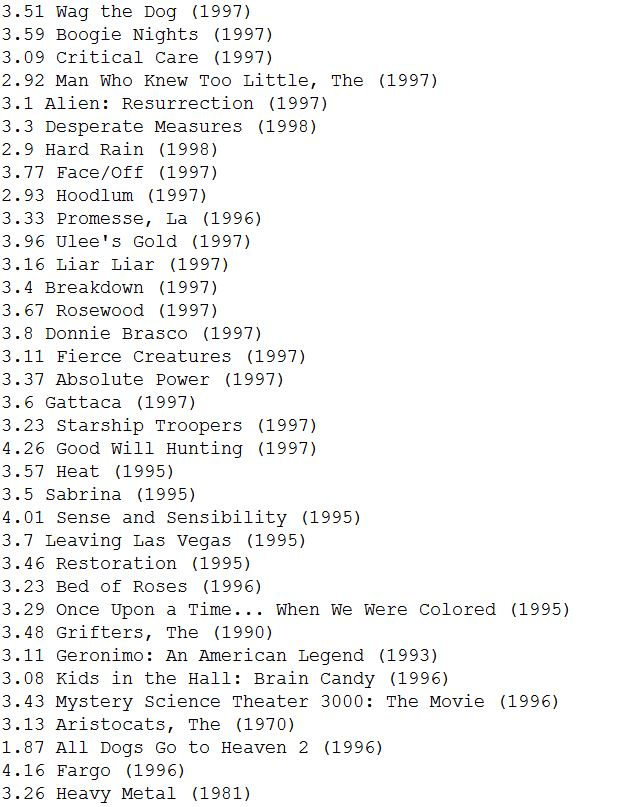
\includegraphics[scale=0.55, keepaspectratio=true]{figures/2.JPG}
\caption{MovieLense rating}
\label{fig:q5fig1}
\end{center}
\end{figure}
\newpage
\item The output file for IMDB with rating and movie names are in Figure \ref{fig:q5fig2}
\begin{figure}[h!]
\begin{center}
\hspace*{-3cm} 
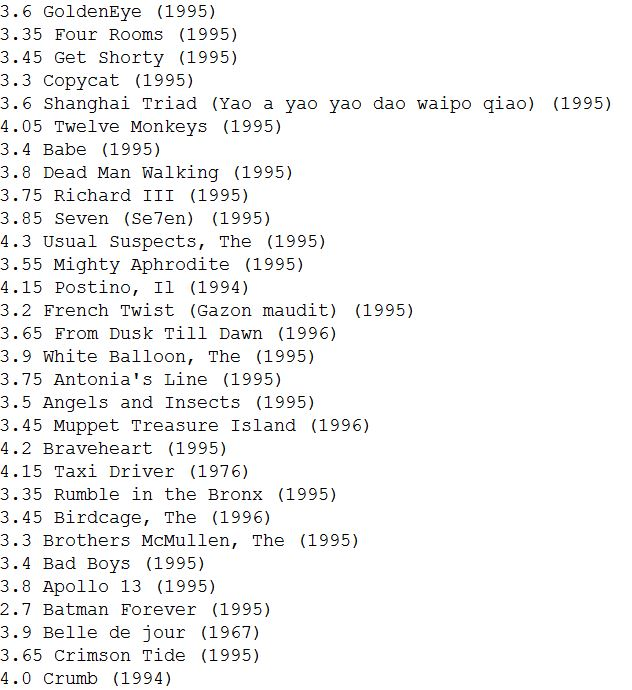
\includegraphics[scale=0.55, keepaspectratio=true]{figures/3.JPG}
\caption{IMDB rating}
\label{fig:q5fig2}
\end{center}
\end{figure}
\end{itemize}

\newpage
\textbf{Code Listing}
\sloppy
\lstinputlisting[language=Python,caption=Python code for ranking movies based on MovieLense data.,frame=single,breaklines=true,label=lst:q5code1, tabsize=2, captionpos=b,numbers=left,showspaces=false,showstringspaces=false,basicstyle=\footnotesize]{src/rankBasedOmovieLense.py}

\newpage
\textbf{Code Listing}
\sloppy
\lstinputlisting[language=Python,caption=Python code for ranking movies based on IMDB data.,frame=single,breaklines=true,label=lst:q5code2, tabsize=2, captionpos=b,numbers=left,showspaces=false,showstringspaces=false,basicstyle=\footnotesize]{src/getIMDB.py}